\chapter[Implementation and Integration of an ASDF Library]
{Implementation and Integration\\of an ASDF Library}
\label{sec:implementation}

The development of the Audio Scene Description Format (ASDF) has been described
in chapter~\ref{sec:format-development}
and its full specification and documentation can be found
in appendix~\ref{sec:asdf}.
However, a file format is only useful if there is software available
that can load files with that format.
Therefore, a software library\footnote{%
\url{https://github.com/AudioSceneDescriptionFormat/asdf-rust}}
has been implemented as well, using the Rust\footnote{%
\url{https://www.rust-lang.org/}} programming language.
The following sections describe the implementation of this library.
A library alone is still not enough to listen to audio scenes,
it also has to be integrated into a software that is able to reproduce
those audio scenes.
The ASDF library has been integrated in a standalone rendering software
(see section~\ref{sec:integration-ssr})
and in a plugin for a visual programming language for multimedia
(see section~\ref{sec:integration-pd}).
These integrations use the C language interface of the ASDF library
which makes it easy to integrate with software written in other languages.


\section{ASDF Parsing}

The ASDF syntax is based on XML.
An existing XML parser library\footnote{%
\url{https://crates.io/crates/xmlparser}}
is used to load ASDF files.
The XML library automatically checks whether a file is well-formed XML,
but the conformance to ASDF syntax is checked manually.
Manual validation makes it easier to provide helpful error messages
in case an erroneous ASDF file is provided.
It is important to provide informative and very specific error messages
to help scene authors to create working scenes quickly.
For example,
the following small scene is well-formed and valid XML,
but it still contains an error:

\input{highlighted-code/broken-scene.asd}

\noindent
When trying to load this audio scene
-- assuming the referenced audio file indeed does not exist --
the ASDF library would provide this error message:

\input{highlighted-code/broken-scene-error1.txt}

\noindent
If the audio file is changed to one that exists,
but has only one channel,
a different error will be raised:

\input{highlighted-code/broken-scene-error2.txt}

\noindent
Showing the affected part of the scene within the error message
should help localizing the cause of the error more quickly,
especially in a non-trivial scene
that is much larger than this minimalistic example.


\section{Audio File Playback}
\label{sec:audio-file-playback}

The ASDF library allows playback of
WAV, OGG (Vorbis), FLAC and MP3 sound files.
It is not feasible to load all sound files of a scene
in their entirety into memory.
A scene might contain many very long files
that are supposed
to be played at the same time.
It is sufficient to provide the audio data in small blocks.
At any time during playback, though,
the appropriate parts of the currently active sound files
have to be provided to the rendering software
within a very short time.
Otherwise, the output signal could be interrupted,
leading to audible artifacts.
To avoid this,
a certain amount of data from all relevant audio files is buffered,
which makes sure that there are no excessive delays
when reading and decoding the files.
The buffering happens in a separate thread
which runs in parallel to the audio processing,
and typically with a lower priority.
This parallel processing in multiple threads
is traditionally very error-prone.
This was the
main reason why the programming language Rust was chosen
to implement the library.
Rust allows the implementation of very efficient programs
that are still safe in the presence of multiple threads.

An additional requirement that complicates the implementation
is that a user should be able to \emph{seek} forward and backward
in a scene.
It should be possible to jump to any time within the timeline of a scene.
When that happens,
playback is stopped, all existing buffers are discarded, new buffers are filled
with the audio data that is to be played back at the new time instance
and finally playback is resumed at the desired point in time.

Different audio files in a scene can have different sampling rates,
which could again be different from the output sampling rate of the reproduction
software.
In case of a mismatch, audio data is automatically re-sampled.


\section{Transforms}

As explained in chapter~\ref{sec:development-transforms},
so-called \emph{transforms} are used to define spatial
positions of objects and to change positions and orientations over time.
When a sequence of positions and/or orientations and/or volume values
is given in a transform, \emph{splines} are created
based on the given control values.
A separate Rust library\footnote{%
\url{https://github.com/AudioSceneDescriptionFormat/asdfspline-rust}}
has been implemented to provide all necessary types of splines.
Within the main ASDF library,
all transforms -- including their splines -- are created when loading
an ASDF file and they are stored for quick retrieval by the IDs they are
applying to.

Whenever the transform of a source (or of the listener) is requested
for a given time,
it is checked whether there are any transforms applying to its ID.
Only for those transforms that are active at the given time,
it is recursively checked for other transforms applying to them.
Each transform represents a local coordinate system
and all those nested transforms are combined into a final transform.
If a transform contains both a translation and a rotation,
the rotation is applied first.
When multiple transforms apply to the same ID,
only one of them is allowed to have a rotation,
because the order of rotations would be ambiguous.
This is checked when loading a scene and an error is raised
if there are multiple rotations at the same level.
A transform is not allowed to apply to itself, directly or indirectly.
This is also checked when loading the scene.


\section{API}

The interface of the library,
often called Application Programming Interface (API),
allows to choose a scene file to load and to specify a few rendering options
like the sampling rate and block size.
After loading the scene, two main types of data are provided:
audio signals of sound sources and their spatial transforms.
The spatial transform of the listener's position (also called \emph{reference})
is also available.

Audio data is provided in fixed-size blocks with the given block size
and with as many channels as there are sources in the scene.
If a source is not active at a given time, its signal consists of all zeros.
Each audio block is provided immediately,
thanks to the buffering described
in section~\ref{sec:audio-file-playback} above,
which enables glitch-free playback.

It is also possible to \emph{seek} in a scene,
in other words, to jump to a different point in time.
In this case, the next audio block is faded out
and some empty audio blocks are delivered during buffering.
Once the buffers are filled, the next audio block is faded in and
playback continues at the new scene time.

While the audio data is provided in consecutive blocks,
the spatial transform for any source (or for the reference)
can be queried at any desired scene time.
Typically, a rendering application will obtain the transforms
once per audio block and interpolate or cross-fade
from the previous values to the current values.
However, it is possible to query the values at a higher or a lower rate,
if desired.
It is theoretically possible to query the transform values
at every audio sample,
but this will lead to a high computational load.
The library is providing a transform value for each queried time instance,
even if the value did not change compared to the previous query.
If needed, the host application can filter out repeated values.
This is done in the Pure Data external, see section~\ref{sec:integration-pd}.

Since the ASDF library is implemented in Rust,
it can be easily used in any Rust program.
However, having only a Rust API would severely limit the possible use cases.
Therefore, C language bindings have been implemented 
using a widely used tool\footnote{\url{https://github.com/lu-zero/cargo-c}}
from the Rust ecosystem.
This extends the potential uses of the ASDF library to applications written in
C (see section~\ref{sec:integration-pd}),
C++ (see section~\ref{sec:integration-ssr})
and a myriad of other languages.


\section{Integration in a Standalone Rendering Application}
\label{sec:integration-ssr}

The development of the ASDF happened in the context of
a spatial audio rendering tool called SoundScape Renderer (SSR)\footnote{%
\url{http://spatialaudio.net/ssr/}}
\parencite{geier2007ssr,geier2008ssr,geier2012spatial}.
The SSR was co-developed with Jens Ahrens and several collaborators\footnote{%
\url{https://ssr.readthedocs.io/general.html\#contributors}}.
The SSR can be used to render an audio scene with several reproduction methods,
including dynamic binaural rendering, Wave Field Synthesis (WFS) and Higher-Order Ambisonics (HOA).
It is based on an efficient multi-threaded rendering architecture
\parencite{geier2012apf}
and it can be used both as a standalone application and
as \emph{externals} for Pure Data\footnote{\url{https://puredata.info/}}.

As part of the development of the ASDF,
the ASDF library has been integrated into the SSR.
At the time of writing,
binaural rendering is
the only three-dimensional reproduction method,
the other rendering methods are limited to the horizontal plane.
The default graphical user interface is also still limited to the horizontal
plane,
but an experimental three-dimensional user interface is also available,
see section~\ref{sec:visualization}.

The SSR uses the JACK\footnote{\url{https://jackaudio.org/}}
audio server for the handling of audio signals.
The audio file playback of the ASDF library
has been integrated with the
JACK \emph{transport} mechanism
using the \emph{seek} functionality mentioned in
section~\ref{sec:audio-file-playback}.
This way it is possible to play ASDF scenes in synchrony
with other JACK-enabled applications.


\section{Integration as an External for Pure Data}
\label{sec:integration-pd}

\begin{figure}
\centering
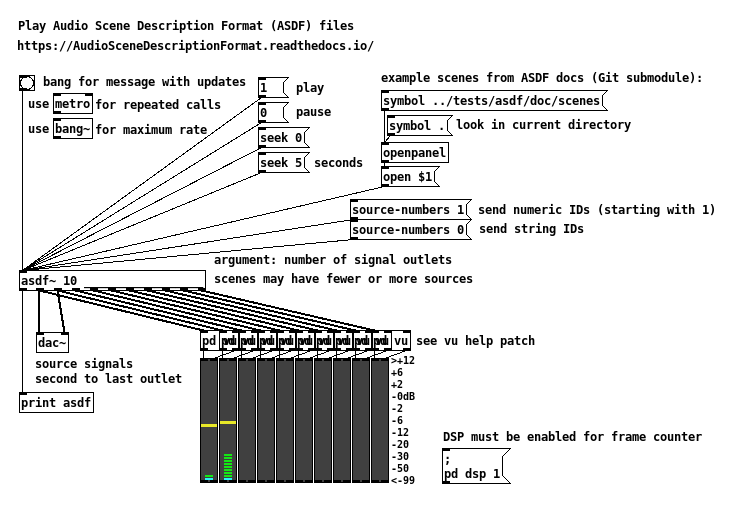
\includegraphics[scale=0.5]{images/asdf-help-pure-data-screenshot}
\caption{Help patch of the \emph{\code{asdf\textasciitilde}} external for Pure Data}
\label{fig:asdf-help-pure-data-screenshot}
\end{figure}

The ASDF library implementation contains\footnote{%
\url{https://github.com/AudioSceneDescriptionFormat/asdf-rust/tree/master/pure-data}}
an \emph{external} for
Pure Data\footnote{\url{https://puredata.info/}}
as a usage example for the C interface.
Figure~\ref{fig:asdf-help-pure-data-screenshot}
shows a screenshot of the external's help patch.
The number of signal outlets has to be provided when creating the external.
Only that number of source signals are provided,
even if more sources are defined in the scene.
Playback of the scene can be started and stopped at any time
and it is possible to \emph{seek} to any point in time in the scene.
The transforms of all sources and the listening position
are not automatically provided at the message outlet,
but they can be triggered at any time
by sending a \emph{bang} message to the external.
However,
all values that have not changed
since the last request
are filtered out.

Given the signals for each source and the corresponding messages
with transform updates,
any means of spatialization available in Pure Data
can be used to auralize a scene.
One possibility are the renderer externals provided by the SSR,
see section~\ref{sec:integration-ssr}.
The messages sent by the ASDF external
happen to be compatible with the SSR externals,
the two just have to be connected.
Both the ASDF and SSR externals can be installed
from Pure Data's built-in package manager.


\section{Visualization}
\label{sec:visualization}

\begin{figure}
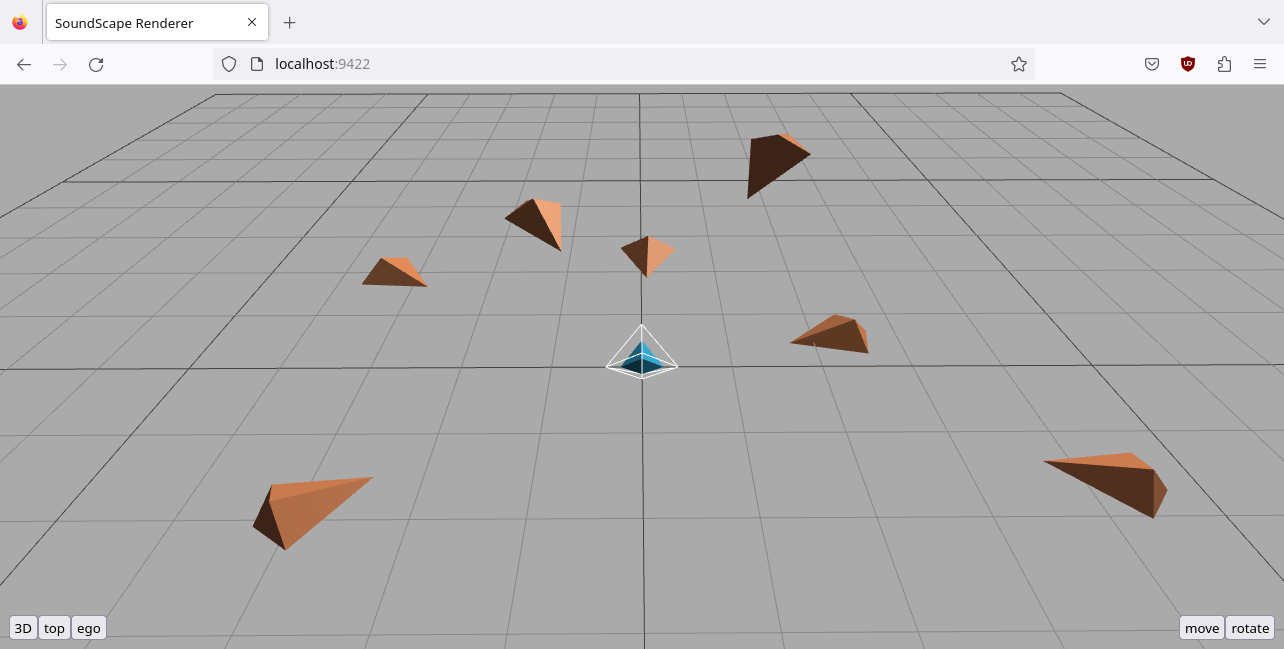
\includegraphics[width=\textwidth]{images/browser-gui-screenshot}
\caption{Screenshot of the browser-based 3D GUI prototype}
\label{fig:browser-gui-screenshot}
\end{figure}

The ASDF is -- as its name suggests --
an audio-only format with no visual aspects.
Nevertheless, it is really helpful for scene authors
to see a visual representation of the sound sources
in the audio scene they are creating.
The ASDF library itself has no capabilities for visualization,
but to aid the development of the ASDF,
a tool for three-dimensional visualization
has been developed for the SoundScape Renderer
(see section~\ref{sec:integration-ssr}).
The tool has been implemented using the
WebGL-based JavaScript library three.js\footnote{\url{https://threejs.org/}}.
More specifically,
it is based on the three.js
editor\footnote{\url{https://threejs.org/editor/}}.
This makes it easy to create a quick prototype
for a three-dimensional user interface
that can be displayed with any modern browser.
The communication with the SSR takes place over the WebSocket protocol,
which is supported by all modern browsers.
A screenshot of web browser displaying an audio scene
is shown in figure~\ref{fig:browser-gui-screenshot}.

The visualization is quite basic and there are many desirable features that are
missing, but it is already possible to get an idea about the three-dimensional
movements of scene objects while the scene is playing.


\section{Example Scenes}

Many minimalistic scenes are available in the ASDF documentation,
see appendix~\ref{sec:asdf}.
Some larger example scenes are available for download from the ASDF development
pages\footnote{%
\url{https://github.com/AudioSceneDescriptionFormat/asdf-example-scenes}}.
